% !TEX root = ../SegwayDoku.tex
\renewcommand{\autoren}{Severin Schendel	}
%\newpage
\subsection{Vergleich der Antriebsarten}
\subsubsection{Bürstenloser Gleichstrommotor}

\begin{quote}
"Bürstenlose Gleichstrommotoren, kurz BLDC („Brushless DC-Motoren), sind -  entgegen ihrer Bezeichnung - Drehstrom-Synchronmaschinen: Der Läufer folgt einem magnetischen Drehfeld, die Bewegung ist synchron zur Wechselspannung, die an die Wicklungen angelegt wird. Dieser Motortyp wird häufig als „Bürstenloser Gleichstrommotor“ bezeichnet, da er in vielen Applikationen bürstenbehaftete Gleichstrommotoren („brushed DC“, Kommutatormotoren) ersetzt. Bei einem bürstenbehafteten Gleichstrommotor wird eine Gleichspannung angelegt, die durch einen mechanischen Wechselrichter im Motor - die Bürsten - einen drehzahlunabhängigen Wechselstrom erzeugt.

Zusammen mit einer elektronischen Ansteuerung, die die Funktion der Bürsten übernimmt und aus den eingespeisten Gleichstrom in Wechselstrom umwandelt, entspricht der BLDC-Motor im Verhalten einem bürstenbehafteten Gleichstrommotor ohne die in der Lebensdauer begrenzten Bürsten.  BLDC-Motoren werden deshalb auch als EC („electronically commutated“)-Motoren bezeichnet, um sie von mechanisch kommutierten bürstenbehafteten Motoren abzugrenzen."
\end{quote}
(Quelle: \cite{BLDCNanotec})
\begin{figure}[h]  % [h] bedeutet, dass das Bild genau an dieser Stelle im Text erscheint
\centering\includegraphics[width=0.7\textwidth]{images/BLDC_Prinzipschaltung}
\caption{BLDC Prinzipschaltung, V1-V6 MOSFETS \newline (Quelle: \cite{PrinzipBLDC})}
\label{PrinzipBLDC}
\end{figure}
\newpage
